% Created 2018-03-13 mar 13:26
\documentclass[a4paper]{scrartcl}
\usepackage[utf8]{inputenc}
\usepackage[T1]{fontenc}
\usepackage{fixltx2e}
\usepackage{graphicx}
\usepackage{longtable}
\usepackage{float}
\usepackage{wrapfig}
\usepackage{rotating}
\usepackage[normalem]{ulem}
\usepackage{amsmath}
\usepackage{textcomp}
\usepackage{marvosym}
\usepackage{wasysym}
\usepackage{amssymb}
\usepackage{hyperref}
\tolerance=1000
\usepackage{khpreamble}
\newcommand*{\shift}{\operatorname{q}}
\author{Kjartan Halvorsen}
\date{Due 2018-03-07}
\title{Computerized control - homework 3}
\hypersetup{
  pdfkeywords={},
  pdfsubject={},
  pdfcreator={Emacs 24.5.1 (Org mode 8.2.10)}}
\begin{document}

\maketitle

\section*{The system}
\label{sec-1}
Consider the linearized model of the tank that we looked at in class

\begin{center}
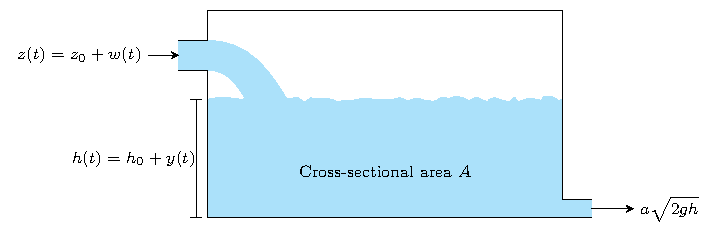
\includegraphics[width=0.7\linewidth]{../../MR2012/figures/tank-with-hole}
\end{center}
Using the parameter values 
\[ A = 1, \qquad a = 0.1, \qquad g = 9.8,\]
and the operating point given by
\[ h_0 = 1, \qquad z_0 = a\sqrt{2gh_0} \approx 0.44,\]
the linearized model of the tank is described by the first-order system
\[ G_1(s) = \frac{1}{s + 0.44}\]
from the deviation in flow $w(t)$ to the deviation in level $y(t)$.

A valve is used to control the flow. The valve is a so-called control valve, which means it includes an inner controller that works as a position servo. That is, it will make sure the opening of the valve follows the input signal to the valve. This signal is named $u(t)$. The response of the opening of the valve $\theta(t)$ to the input signal $u(t)$ is well-described by a second-order, critically damped system
\[ G_2(s) = \frac{1}{(0.5s + 1)(0.5s+1)} = \frac{4}{(s+2)(s+2)}. \]

The flow through the valve depends also on the square root of the pressure difference across the valve. In a linearized model, a change in pressure enters as an additive disturbance to the system. The complete model of the process is given in the block-diagram below.

  \begin{center}
  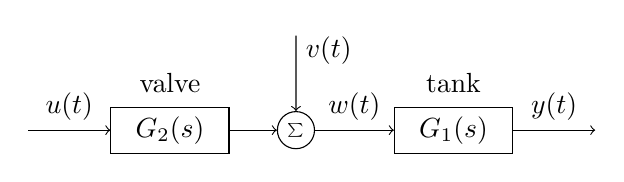
\begin{tikzpicture}[scale = 0.8, node distance=18mm, block/.style={rectangle, draw, minimum width=15mm}, sumnode/.style={circle, draw, inner sep=2pt}]
  
  \node[coordinate] (input) {};
  \node[block, right of=input] (valve) {$G_2(s)$};
  \node[above of=valve, node distance=6mm] {valve};
  \node[sumnode, right of=valve, node distance=16mm] (sum) {\tiny $\sum$};
  \node[block, right of=sum, node distance=20mm] (tank) {$G_1(s)$};
  \node[above of=tank, node distance=6mm] {tank};
  \node[coordinate, right of=tank] (output) {};
  \node[coordinate, above of=sum, node distance=12mm] (disturbance) {};

  \draw[->] (input) -- node[above] {$u(t)$} (valve);
  \draw[->] (valve) -- node[above] {} (sum);
  \draw[->] (sum) -- node[above] {$w(t)$} (tank);
  \draw[->] (tank) -- node[above] {$y(t)$} (output);
  \draw[->] (disturbance) -- node[right, pos=0.2] {$v(t)$} (sum);

  \end{tikzpicture}
\end{center}

The level of the tank is measured, and is available for feedback control. 
    \begin{center}
  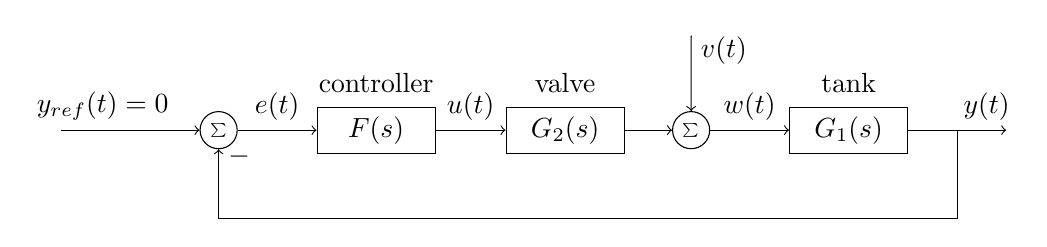
\begin{tikzpicture}[scale = 0.8, node distance=20mm, block/.style={rectangle, draw, minimum width=15mm}, sumnode/.style={circle, draw, inner sep=2pt}]
  
  \node[coordinate] (refinput) {};
  \node[sumnode, right of=refinput, node distance=20mm] (sumerr) {\tiny $\sum$};
  \node[block, right of=sumerr] (controller) {$F(s)$};
  \node[above of=controller, node distance=6mm] {controller};
  \node[block, right of=controller, node distance=24mm] (valve) {$G_2(s)$};
  \node[above of=valve, node distance=6mm] {valve};
  \node[sumnode, right of=valve, node distance=16mm] (sum) {\tiny $\sum$};
  \node[block, right of=sum, node distance=20mm] (tank) {$G_1(s)$};
  \node[above of=tank, node distance=6mm] {tank};
  \node[coordinate, right of=tank, node distance=20mm] (output) {};
  \node[coordinate, above of=sum, node distance=12mm] (disturbance) {};

  \draw[->] (refinput) -- node[above, pos=0.3] {$y_{ref}(t)=0$} (sumerr);
  \draw[->] (sumerr) -- node[above] {$e(t)$} (controller);
  \draw[->] (controller) -- node[above] {$u(t)$} (valve);
  \draw[->] (valve) -- node[above] {} (sum);
  \draw[->] (sum) -- node[above] {$w(t)$} (tank);
  \draw[->] (tank) -- node[coordinate] (measure) {} node[above, pos=0.8] {$y(t)$} (output);
  \draw[->] (disturbance) -- node[right, pos=0.2] {$v(t)$} (sum);
  \draw[->] (measure) -- ++(0,-14mm) -| node[right, pos=0.95] {$-$} (sumerr);
 \end{tikzpicture}
\end{center}


A simulation model (\texttt{simulink}) of the system is available on Blackboard under \texttt{Course Documents/Matlab and Simulink} 

\section*{Exercises}
\label{sec-2}
\subsection*{Problem 1 - Tuning a PID}
\label{sec-2-1}

Perform a bumptest on the plant (valve+tank). This means to connect a step block (see \texttt{Sources} in the \texttt{Simulink Library Browser}) to the input of the valve. Determine the slope $R$, the apparent deadtime $L$, and the parameter $a=RL$ from the step response. See figure 8.13 in the text-book

\begin{center}
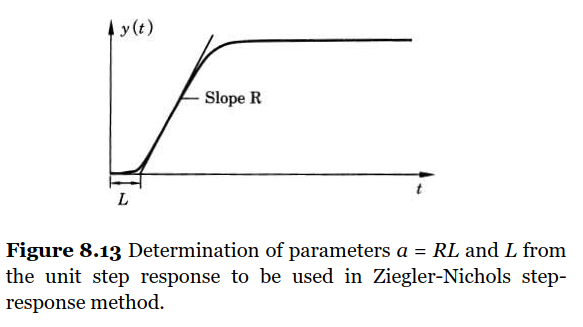
\includegraphics[width=0.7\linewidth]{../figures/fig8-13.png}
\end{center}

Include your simulated step-response in your report.

Determine a PID controller using table 8.2 in the book.

\begin{center}
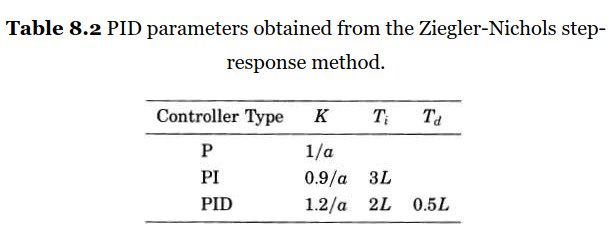
\includegraphics[width=0.7\linewidth]{../figures/table8-2.png}
\end{center}

\subsection*{Problem 2 - Implement the PID in simulink}
\label{sec-2-2}

The controller is written
\[U(s) = K \left( U_c(s) - Y(s) + \frac{1}{sT_i}\big(U_c(s) - Y(s)\big) - \frac{sT_d}{1 + sT_d/N} Y(s)\right).\]

Set $N=10$ and implement the controller in simulink using the values for $K$, $T_i$ and $T_d$ that you determined in Problem 1.

Simulate the closed-loop system's response to step changes in both the set point, $u_c(t)$ and the disturbance, $v(t)$. Include the step-responses in your report and comment on the results.

\subsection*{Problem 3 - Discrete PID}
\label{sec-2-3}

The discretized controller is written
\[ R(\shift) u(kh) = T(\shift) u_c(kh) - S(\shift) y(kh), \]
where
\begin{align*}
 R(\shift) &= (\shift -1)(\shift - a_d)\\
 S(\shift) &= s_0\shift^2 + s_1\shift + s_2\\
T(\shift) &= t_0\shift^2 + t_1\shift + t_2
\end{align*}

Determine the discrete PID controller parameters $a_d$, $s_0$, $s_1$, $s_2$, $t_0$, $t_1$ and $t_2$ using table 8.1 in the textbook (given below). You can use whichever of the three discretization methods provided.

\begin{center}
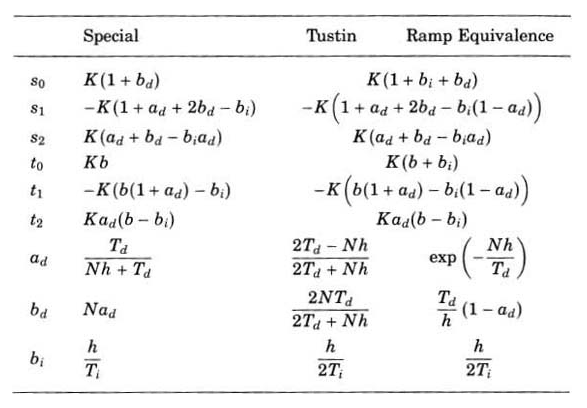
\includegraphics[width=0.7\linewidth]{../figures/table8-1.png}
\end{center}

\section*{Solutions}
\label{sec-3}
\subsection*{Problem 1 - Tuning a PID}
\label{sec-3-1}

Below is the result from a bumptest on the plant (valve+tank).
\begin{center}
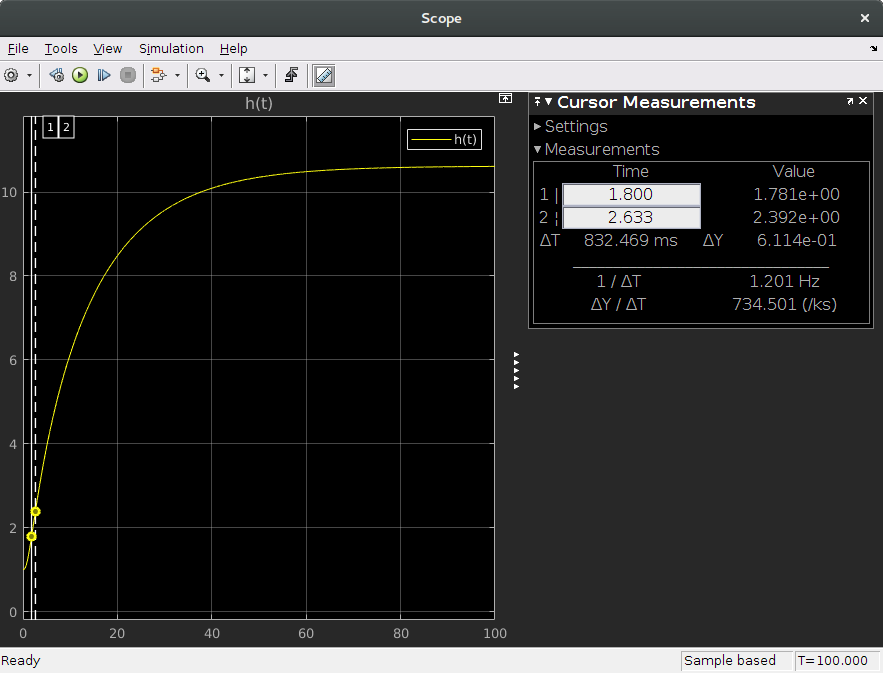
\includegraphics[width=0.7\linewidth]{./figures/hw3-bumptest.png}
\end{center}
The measurement points (\(t_1, y_1\)) and (\(t_2, y_2\)) were moved around in order to find two close points which gave the largest slope \(R = \frac{y_2-y_1}{t_2-t_1}\). The apparent deadtime $L$ is the intersection of the steepest tangent with the time axis. This can be found by noting that if we take the midpoint of $y_1$ and $y_2$ as the tangent point, then $R = \frac{y_2+y_1}{2L}$. We get
\begin{align*}
R &= \frac{y_2-y_1}{t_2-t_1} = 0.73\\
L &= \frac{y_1+y_2}{2R} = 2.85\\
a &= RL = 2.09
\end{align*}

From table 8.2 we obtain the parameters
\begin{align*}
K &= 1.2/a = 0.575\\
T_i &= 2L = 5.69\\
T_d &= 0.5L = 1.42
\end{align*}

\subsection*{Problem 2 - Implement the PID in simulink}
\label{sec-3-2}

The controller is written
\[U(s) = K \left( U_c(s) - Y(s) + \frac{1}{sT_i}\big(U_c(s) - Y(s)\big) - \frac{sT_d}{1 + sT_d/N} Y(s)\right).\]

In \texttt{simulink} the model should look like the following
\begin{center}
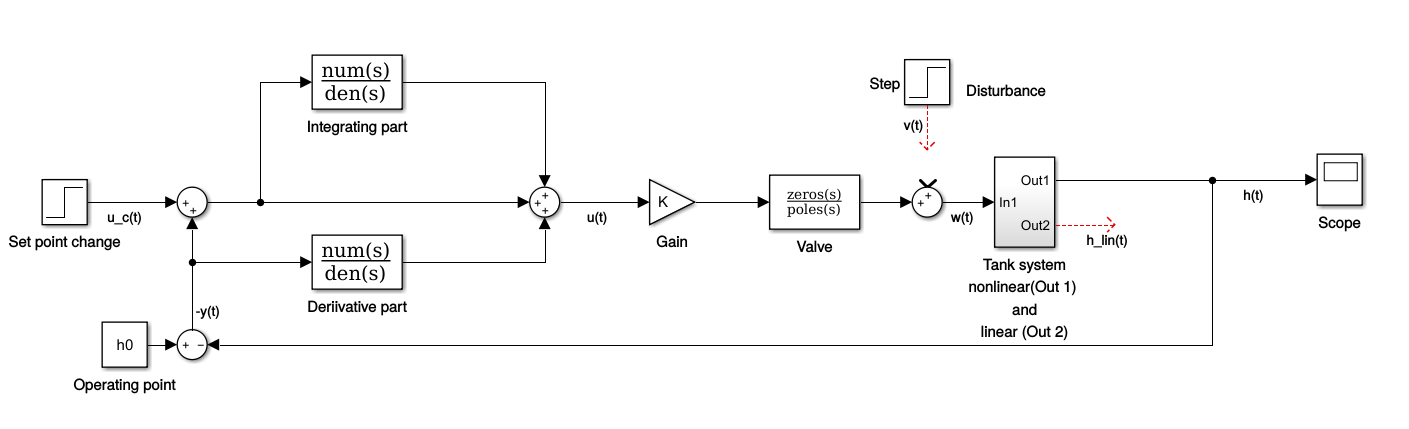
\includegraphics[width=0.9\linewidth]{./figures/hw3-pid-block.png}
\end{center}
Note that the derivative part acts only on the feedback signal $-y(t)$. The blocks are
\begin{description}
\item[{Derivative part}] num: [Td, 0], den: [Td/N, 1]
\item[{Integrating part}] num: [ 1 ], den: [Ti, 0]
\end{description}

A step response of the closed-loop system is given below. A step change in the set point occurs at time $t=10$ and then a step in the disturbance occurs at time $t=50$. 
\begin{center}
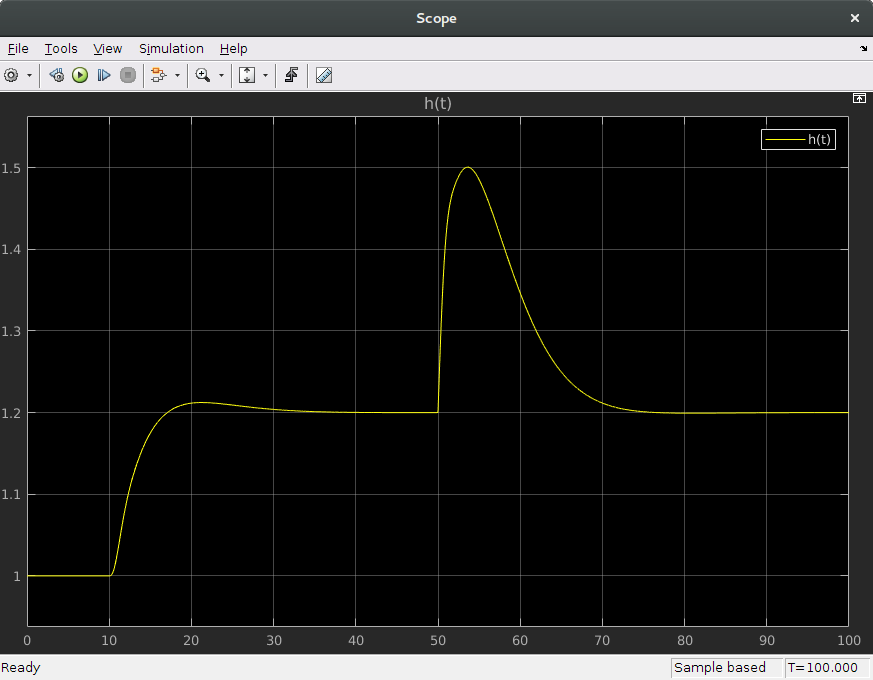
\includegraphics[width=0.6\linewidth]{./figures/hw3-pid-step.png}
\end{center}

We can see that thanks to the integrating part of the controller, there is no steady-state error. It takes the system about 20 seconds to settle. There is some overshoot in the set-point response, but not too much. This should be acceptable. 

\subsection*{Problem 3 - Discrete PID}
\label{sec-3-3}

The discretized controller is written
\[ R(\shift) u(kh) = T(\shift) u_c(kh) - S(\shift) y(kh), \]
where
\begin{align*}
 R(\shift) &= (\shift -1)(\shift - a_d)\\
 S(\shift) &= s_0\shift^2 + s_1\shift + s_2\\
T(\shift) &= t_0\shift^2 + t_1\shift + t_2
\end{align*}

Determine the discrete PID controller parameters $a_d$, $s_0$, $s_1$, $s_2$, $t_0$, $t_1$ and $t_2$ using table 8.1 in the textbook (given below). 

Using the special discretization (and $b=1$) we get

\begin{align*}
  a_d &= \frac{T_d}{Nh + T_d} = \frac{1.42}{10h + 1.42}\\
  s_0 &= K(1 + b_d) = K(1 + Na_d) = 0.575(1 + \frac{14.2}{10h + 1.42})\\
  s_1 &= -K(1 + a_d + 2b_d - b_i) = -0.575( 1 + \frac{1.42 + 28.4}{10h + 1.42} - \frac{h}{5.69})\\
  s_2 &= K(a_d + b_d - b_ia_d) = 0.575\frac{1.42 + 14.2 - h/5.69}{10h + 1.42}\\
  t_0 &= Kb = 0.575\\
  t_1 &= -K(b(1+a_d) - b_i) = -0.575( \frac{10h + 1.42 + 1.42}{10h + 1.42} - \frac{h}{5.69})\\
  t_2 &= Ka_d(b-b_i) = 0.575 \frac{1.42(1-\frac{h}{5.69})}{10h + 1.42}
\end{align*}
% Emacs 24.5.1 (Org mode 8.2.10)
\end{document}